% !TEX TS-program = pdflatex
% !TEX encoding = UTF-8 Unicode

% This is a simple template for a LaTeX document using the "article" class.
% See "book", "report", "letter" for other types of document.

\documentclass[12pt]{article} % use larger type; default would be 10pt
\linespread{1.6} % `double' spacing

\usepackage[utf8]{inputenc} % set input encoding (not needed with XeLaTeX)

%%% Examples of Article customizations
% These packages are optional, depending whether you want the features they provide.
% See the LaTeX Companion or other references for full information.

%%% PAGE DIMENSIONS
\usepackage{geometry} % to change the page dimensions
\geometry{a4paper} % or letterpaper (US) or a5paper or....
% \geometry{margin=2in} % for example, change the margins to 2 inches all round
% \geometry{landscape} % set up the page for landscape
%   read geometry.pdf for detailed page layout information

\usepackage{graphicx} % support the \includegraphics command and options

% \usepackage[parfill]{parskip} % Activate to begin paragraphs with an empty line rather than an indent

%%% PACKAGES
\usepackage{booktabs} % for much better looking tables
\usepackage{array} % for better arrays (eg matrices) in maths
\usepackage{paralist} % very flexible & customisable lists (eg. enumerate/itemize, etc.)
\usepackage{verbatim} % adds environment for commenting out blocks of text & for better verbatim
\usepackage{subfig} % make it possible to include more than one captioned figure/table in a single float
% These packages are all incorporated in the memoir class to one degree or another...

%%% HEADERS & FOOTERS
\usepackage{fancyhdr} % This should be set AFTER setting up the page geometry
\pagestyle{fancy} % options: empty , plain , fancy
\renewcommand{\headrulewidth}{0pt} % customise the layout...
\lhead{}\chead{}\rhead{}
\lfoot{}\cfoot{\thepage}\rfoot{}

%%% SECTION TITLE APPEARANCE
%\usepackage{sectsty}
%\allsectionsfont{\sffamily\mdseries\upshape} % (See the fntguide.pdf for font help)
% (This matches ConTeXt defaults)

%%% ToC (table of contents) APPEARANCE
\usepackage[nottoc,notlof,notlot]{tocbibind} % Put the bibliography in the ToC
\usepackage[titles,subfigure]{tocloft} % Alter the style of the Table of Contents
\renewcommand{\cftsecfont}{\rmfamily\mdseries\upshape}
\renewcommand{\cftsecpagefont}{\rmfamily\mdseries\upshape} % No bold!

% Hyperlinks, URLs etc.
\usepackage{hyperref}
\usepackage{url}
\hypersetup{
    colorlinks=true,
    citecolor=black,
    urlcolor=black,
    linkcolor=black,
    pagecolor=black,
    anchorcolor=black
}

\usepackage{ctable}
\usepackage{csvsimple}

%%% END Article customizations

%%% The "real" document content comes below...

\title{The Channel Tunnel}
\author{Jake Humphrey}
\date{} % Activate to display a given date or no date (if empty),
         % otherwise the current date is printed 

\begin{document}
\maketitle

\section{Introduction}
\label{sec:intro}

The concept of a man-made undersea tunnel connecting England and France has existed since the early 1800s, but it was not until 1986 that the construction effort resulting in the present Channel Tunnel was started.

Since its opening in 1994, the Channel Tunnel, affectionately nicknamed \emph{The Chunnel}, has transported over 300 million passengers and 300 million tonnes of freight between England and France across the English Channel (French: \emph{La Manche}).

As a work of engineering, the Tunnel is rather impressive. The only precedent of its type is the Seikan Tunnel in Japan, which connects the main island of Honsh\={u} with the Northern island of Hokkaid\={o}. The Channel Tunnel comprises two main rail tunnels and one service tunnel between them. The boring itself made use of a stratum of chalk marl, which has properties conducive to tunnelling. All of its achievements have contributed to its designation as one of the Seven Wonders of the Modern World by the American Society of Civil Engineers.

The Channel Tunnel offers both freight and passenger access to separate rail operators, in addition to a roll-on roll-off shuttle service for road vehicles named Eurotunnel Le Shuttle.

This document seeks to give the reader (having a background in an engineering discipline) an overview of the history, construction, and operation of the Channel Tunnel, and an insight into its impact on transport infrastructure and the economy in England and France.

\section{History of Channel Crossing}
\subsection{Planning}

The earliest proposal for connecting England and France beneath the Channel was made by  Albert Mathieu, a French mining engineer, in 1802, and included oil-lamp illumination and an artificial island midway across for changing the horses of one's carriage.\cite{eurotunnel-build}

In 1834 eccentric French engineer and entrepreneur Aimé Thomé de Gamond proposed his first projects for a railway line beneath the English Channel. It was met with indifference from both English and French authorities, who at the time preferred to stay separated from their neighbours.

Gamond presented another proposal to the French Emperor Napoleon III in 1856 detailing a rail line from Cap Gris-Nez to Eastwater Point with a port\slash airshaft on the Varne sandbank. Gamond's preliminary surveying operations had estimated the cost at 170 million francs, or less than £7 million in the money of the time.\cite{ny-gamond}

Gamond proposed a total of seven designs over his lifetime. In 1867 his proposal was finally accepted by Napoleon III and Queen Victoria but was brought to an abrupt end by the Franco-Prussian War of 1870. Sadly, Gamond never saw his dream realised; he died ruined and humiliated in 1876\cite{gamond}

Ironically, this same year an official Anglo-French protocol was established for a cross-Channel railway tunnel\cite{bris}, and in 1881, the Anglo-French Submarine Railway Company conducted preliminary exploratory work on both the English and French sides. A couple of pilot tunnels no longer than 2km each had been dug when the project was abandoned in May 1882, over fears that the tunnel would compromise English national security.

The idea was next brought up nearly 40 years later, after the First World War, at the Paris Peace Conference in 1919, by British Prime Minister David Lloyd George. The suggestion was made as assurance that Britain was willing to defend France in the event of another German attack. However, the proposal was not taken seriously by the French and nothing ever came of it.

Another undeveloped proposal made in 1929 estimated the cost of construction to be about \$150 million. Military concerns of both nations had been addressed in the proposal, which included floodable sections of the tunnel to block access by either side. However, military leaders were not convinced. In addition, some English objected to the \emph{tourism} the project's completion would bring, which would supposedly ruin England's ``splendid isolation'' and ``make England a holiday resort for hordes of more or less undesirable people, who would introduce foreign customs, deface the countryside, and otherwise interrupt English habits of living''.\cite{pop29}

With air power gaining dominance in the military, the effect of a tunnel on national security became less and less significant. In 1955, British and French governments began to support technical and geological surveys. This culminated in a government-funded project to dig twin tunnels, designed to accommodate car shuttle wagons, on either side of a service tunnel. Construction began in 1974, but was cancelled by the British government in January 1975 due to growing concerns over EEC membership and the national economy.

In 1981 British Prime Minister Margaret Thatcher and French President François Mitterand agreed to set up a group, \emph{Eurotunnel} (ET), inviting private companies to put forward propositions. Over the next few years several projects were submitted including a 4.5km suspension bridge holding a road encased in a tube and an undersea drive-through tunnel.

Public opinion favoured the drive-through tunnel, but ventilation issues, concerns about accident management, and fear of driver mesmerisation resulted in the decision of the French and UK governments to facilitate the construction of another proposal: the high-speed rail link proposed by the \emph{Channel Tunnel Group\slash France--Manche} (CTG\slash F--M) consortium.

Eurotunnel absorbed CTG\slash F--M and signed a construction contract with \emph{Transmanche Link}, an international co-operation effort: the five English construction companies forming \emph{Translink Joint Venture} started boring from Shakespeare Cliff, and the five French companies formed \emph{GIE Transmanche} and began from Sangatte.

\begin{figure}[tp]
  \centering
  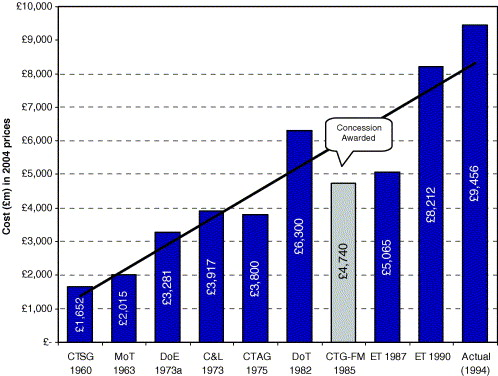
\includegraphics[width=0.8\textwidth]{costproj}
  \caption{Channel Tunnel cost projections.}
  \label{fig:costproj}
\end{figure}

The funding  was of an unprecedented scale for this ambitious project. Eurotunnel's original estimate of £4.7bn doubled to £9.5bn by the end of construction as can be seen in Figure~\ref{fig:costproj}.\cite{costeval} This was in part shareholder investment and partly £8bn of debt which nearly crippled the company in its early years of operation.

\subsection{Construction}
Boring began on February 28 1988. Eleven Tunnel Boring Machines (TBMs), six French and five English, worked from both ends, cutting through a stratum of chalk marl. This material provides high impermeability to water, but easy excavation, and its strength allows for minimal added structural support. The tunnel's path through the geology under the Channel is depicted in Figure~\ref{fig:geo}.

\begin{figure}[tp]
  \centering
  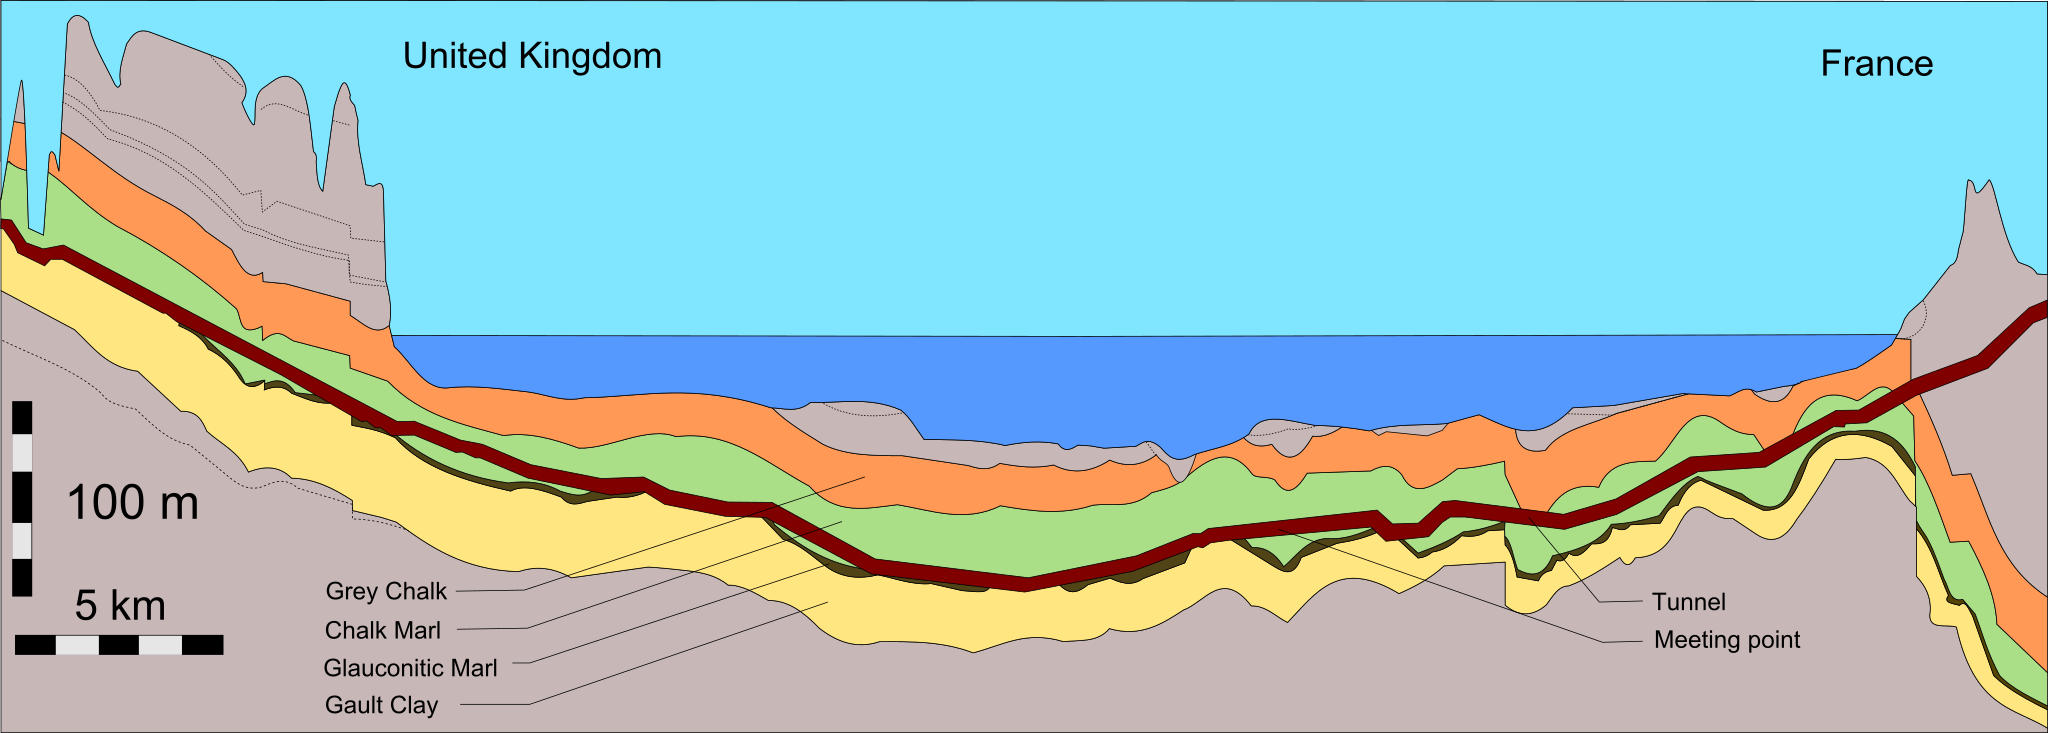
\includegraphics[width=\textwidth]{geology}
  \caption{Channel Tunnel geological profile.}
  \label{fig:geo}
\end{figure}

The tunnelling plan was essentially the same as the cancelled 1975 attempt. The risks taken into account included flooding from the sea above due to weak construction and ground integrity.

The TBMs used combinations of high pressure water jets and rotating disc cutters to burrow at a speed of 75m/day. The central 4.8m-diameter service tunnel was dug first to scout conditions ahead of the two 7.6m-diameter main tunnels. Piston relief ducts connected the rail tunnels to allow for regulation of pressure changes due to the moving trains. A complete cross-section is depicted in Figure~\ref{fig:cross}

The spoil removed from the tunnel was put to use by both sides. The English dumped 4.9m cubic metres of the chalk marl into the sea near Dover, which eventually became Samphire Hoe, a 300,000m$^2$ County Park.\cite{samphoe} The French piled their spoil up to create a new hill.

\begin{figure}[tp]
  \centering
  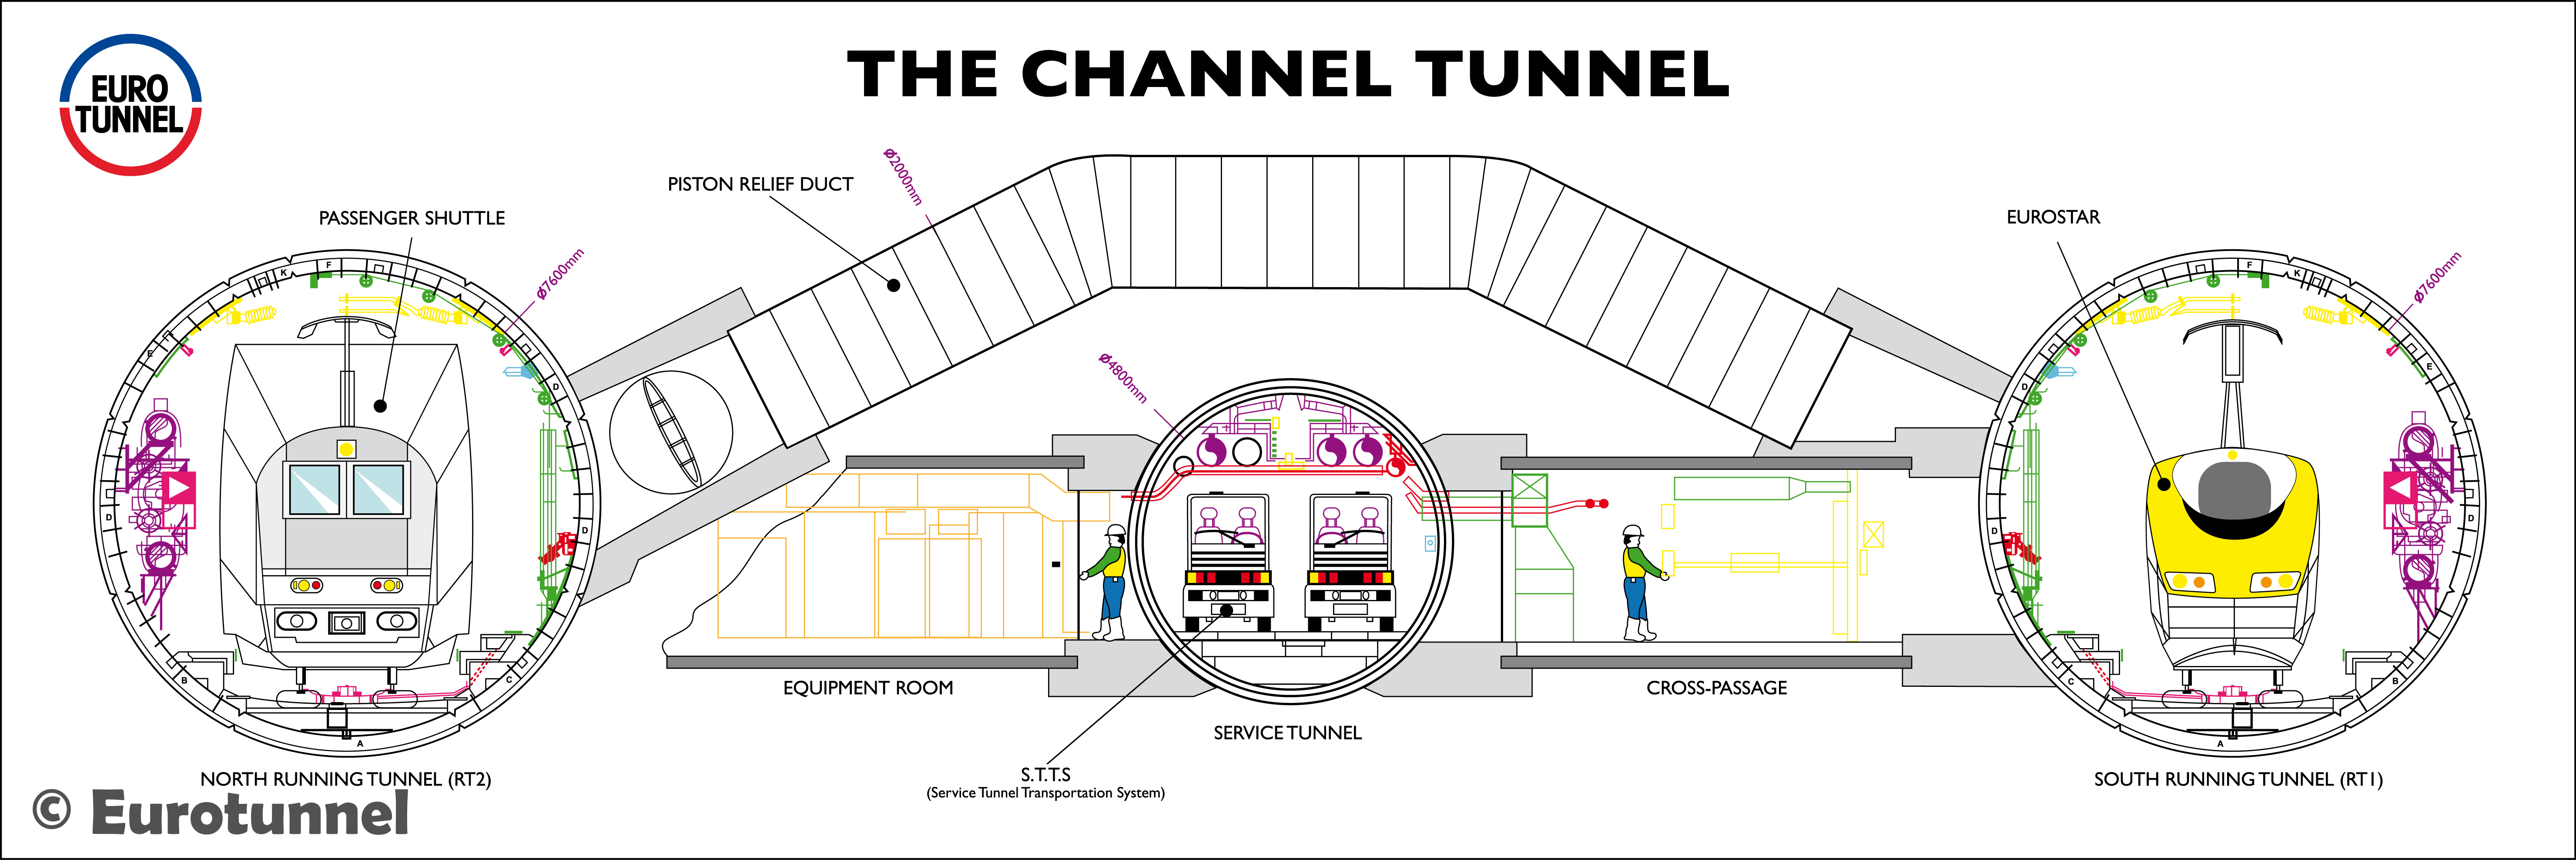
\includegraphics[width=\textwidth]{tunnelcross}
  \caption{Channel Tunnel cross-section.}
  \label{fig:cross}
\end{figure}

The reinforcement strategies differed between the English and French sides. The French used bolted linings of cast iron or high-strength reinforced concrete whereas the English side prioritised speed and thus only applied cast-iron lining in geologically risky areas.

The breakthrough occurred rather unceremoniously on October 30 1990, when a two-inch-diameter pilot hole joined the French and English service tunnels. The official connection of the two tunnels was performed on December 1 1990 by Englishman Graham Fagg and Frenchman Phillippe Cozette, who shook hands through the hole in front of the media.

\begin{figure}[tp]
  \centering
  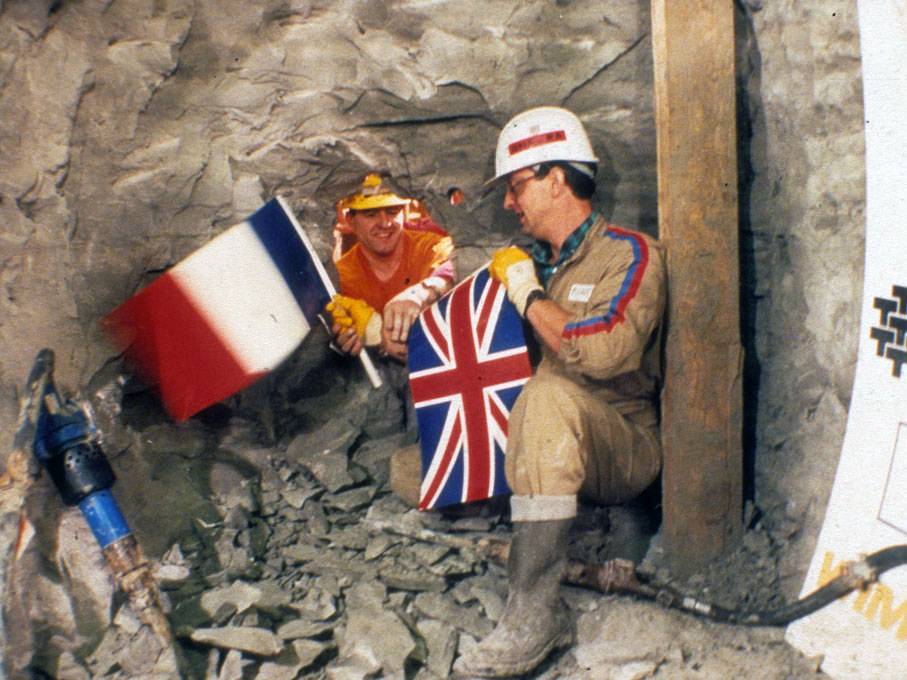
\includegraphics[width=0.8\textwidth]{breakthrough}
  \caption{Englishman Graham Fagg and Frenchman Phillippe Cozette shaking hands through the breakthrough point, December 1 1990.}
  \label{fig:break}
\end{figure}

\begin{figure}[tp]
  \centering
  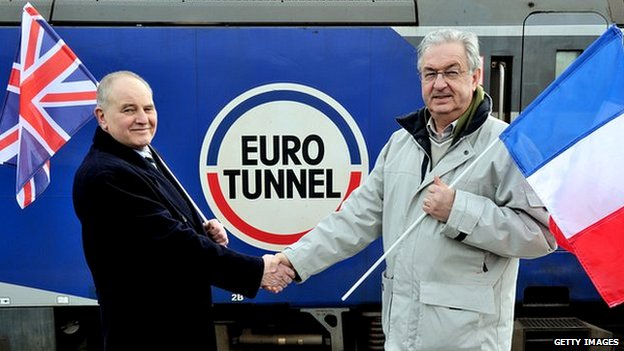
\includegraphics[width=0.8\textwidth]{20years}
  \caption{Englishman Graham Fagg and Frenchman Phillippe Cozette at the 20 year anniversary of the Tunnel's opening.}
  \label{fig:20y}
\end{figure}

The tunnel was completed and the rail service was officially opened on May 6 1994 by Queen Elizabeth II and French President François Mitterand. The full public service commenced several months later.

The railway system boasts two crossover points down the tunnel so that trains can switch tunnels if necessary (This can achieve greater throughputs than simply leaving the two tunnels separate). For signalling, train drivers have displays in the cabs with information which is interconnected with signalling systems on the high-speed connects in both England and France, removing the need to stop and await further information when entering and exiting the tunnel. This advanced cab signalling is also capable of monitoring the train's speed and automatically stopping the train if it goes too fast.

The English end of the Channel Tunnel currently connects to London via the high-speed railway High Speed 1 (completed in 2007). On the French side LGV Nord (\emph{Ligne à Grande Vitesse Nord}, Northern High-speed Line) connects the Tunnel to Lille and then to the Belgian border or to Paris. The electrical power to the Tunnel comes from both English and French sources. An overhead line delivers power to the trains at 25kV 50Hz.

All in all, the Tunnel is 50.5km long and the speed limit is 160km/h, making it traversable in a little under 20 minutes. The Eurostar train service from London to Paris takes about 2h30min, about twice as long as the equivalent journey by air, but significantly cheaper.

\section{Business Operations}
\label{sec:op}

As stated in section~\ref{sec:intro}, there are three services provided by the Channel Tunnel:
\begin{itemize}
	\item Le Shuttle, a shuttle service for road vehicles provided by Channel Tunnel owners Eurotunnel
	\item Passenger trains provided by the international high-speed rail operator Eurostar.\cite{eurostar}
	\item Freight trains operated by DB Schenker Rail (UK).\cite{db-sche}
\end{itemize}

Eurotunnel's commissioned traffic forecasts for the passenger services, which were used to analyse the costs and benefits of building the tunnel, proved to be overly optimistic. Figure~\ref{fig:pass-fore} is taken from an analysis of the Channel Tunnel's fiscal accomplishments made in 2003\cite{costeval}, and it shows that the actual number of passengers ended up only about a half to a third of the forecasted numbers.

\begin{figure}[htp]
  \centering
  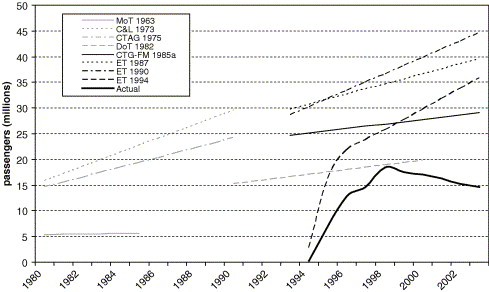
\includegraphics[width=0.8\textwidth]{pass}
  \caption{Channel Tunnel passenger traffic forecasts and actual results (millions of passengers).}
  \label{fig:pass-fore}
\end{figure}

\begin{figure}[htp]
  \centering
  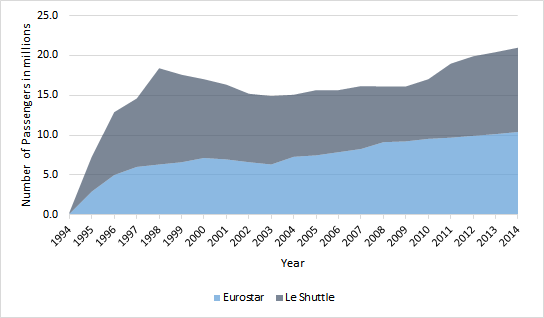
\includegraphics[width=\textwidth]{pass-new}
  \caption{Actual Channel Tunnel passengers, 1994–-2014}
  \label{fig:pass-new}
\end{figure}

The study remarks:
\begin{quote}
\textit{After the opening of the Channel Tunnel, the total number of cross-Channel passengers grew at a considerable pace up until 1998, at which point duty free was abolished. The market then began a process of regression, which continues to the present day.}
\end{quote}

Luckily, as Figure~\ref{fig:pass-new} shows, the market began to improve again after this dip in 2003 due to the Section 1 of High Speed 1's completion. By 2014 the 20m passenger mark had been broken, but this is still far lower than what even the most pessimistic pre-construction forecasts by ET had predicted.

\begin{figure}[htp]
  \centering
  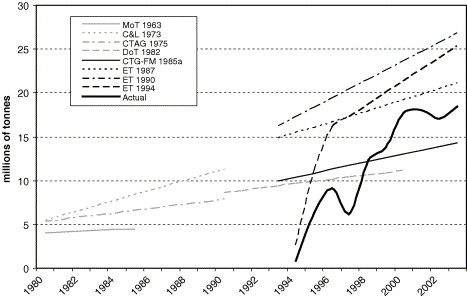
\includegraphics[width=0.8\textwidth]{freight}
  \caption{Channel Tunnel freight forecasts and actual results (million tonnes).}
  \label{fig:freight-fore}
\end{figure}

\begin{figure}[htp]
  \centering
  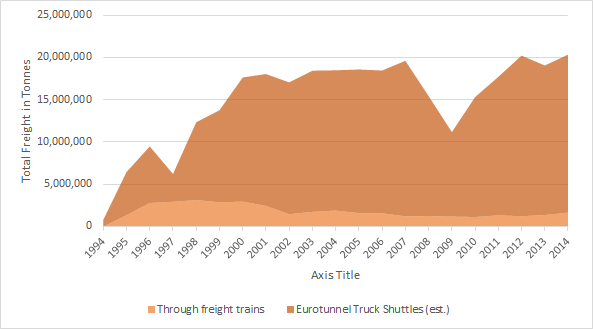
\includegraphics[width=\textwidth]{freight-new}
  \caption{Actual Channel Tunnel freight results, 1994–-2014}
  \label{fig:freight-new}
\end{figure}

The erratic growth patterns of the freight figures compared to forecasts until 2003 can be seen in Figure~\ref{fig:freight-fore}. The drop in 1997 is due to a shuttle fire that closed shuttle service for a time. The volumes passed initial predictions in 1998 and approach 1987 estimates by 2003. They do not, however, reach the updated predictions of 1990 and 1994.

Examining the more recent figures in Figure~\ref{fig:freight-new}, we see that growth has been relatively slow since 2003. Apart from the cutback following another shuttle fire in 2008, numbers have remained largely unchanged, barely surpassing the 20Mt mark in 2014.

Figure~\ref{fig:revenue} shows Eurotunnel's revenue figures taken from their annual reviews\cite{et-reports}, both from their own Le Shuttle service and the money they receive from Eurostar's use of their rail line. This graph closely follows Figure~\ref{fig:pass-new} for the most part, especially in recent years. 

Notable events include the termination of a contract in 2007 which provided Eurotunnel with approximately 70 million Euros per year as a guarantee of minimum income from Eurostar, and in 2012, the liquidation of SeaFrance, a trans-Channel ferry operator, and the redistribution of demand across the market along with acquisition of its assets by Eurotunnel.\cite{et-reports}

\begin{figure}[htp]
  \centering
  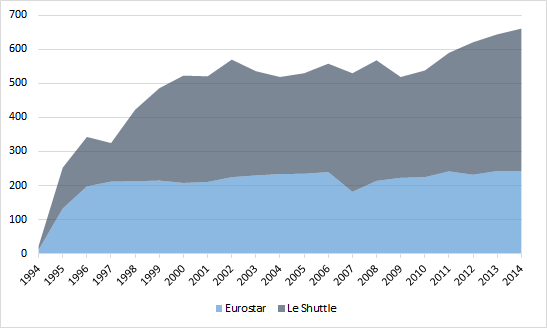
\includegraphics[width=\textwidth]{revenue}
  \caption{Eurotunnel revenue from CT-related sources, 1994–-2014}
  \label{fig:revenue}
\end{figure}

\section{Impact}
In this section the effects of the Channel Tunnel on transport infrastructure and operations in both England and France will be examined.

\subsection{England}
The paper \textit{The Impact of the Channel Tunnel on Kent and Relationsips with Nord-pas-de-Calais} by Hay et al. in 2004\cite{hay04} looks at the effects of the new transport link from an English perspective. According to this paper, UK residents made up 80\%\footnote{So much for ``splendid isolation''!} of cross-Channel travel by any transportation method in 2000.

The opening of the Channel Tunnel and the establishment and success of low-cost airlines in the UK has led to increased competition for cross-Channel travel:
\begin{itemize}
\item Eurotunnel Le Shuttle reached a 50\% market share for cross-Channel car passengers in 2014.
\item In 2011 Eurostar hit 80\% market share for London--Paris--Brussels travel.\cite{star11}
\end{itemize}

These figures show that the Channel Tunnel has firmly established itself as a viable, or even preferred route of cross-Channel travel compared to the air and sea.

According to Hay et al, transport services via the Channel Tunnel have established significant market shares in voyages from England to not only Eurostar-linked France and Belgium, but also Germany and the Netherlands, of which it rested at about 10\% in 2002.

The freight market in the UK is dominated by road travel and the international transport of freight by ferries. With a relatively small airline presence, this left greater potential for the Channel Tunnel to take a larger market share.

There have also been more indirect benefits, such as the image of regions in Kent of being close to high-speed transport links which can help small-medium businesses marketing efforts. For example, \emph{The New Inn} at Etchinghill has rebranded itself as ``The closest pub to the Channel Tunnel''.

Soutetsu Sen points out in the paper \emph{The Channel Tunnel and its impact on Tourism in the United Kingdom}\cite{sen04} that England's privatised rail system meant that the focus was on ``establishing the necessary regulatory structures needed for the tunnel’s construction and operation, rather than ensuring that the regions can fully exploit its opportunities.''

\subsection{France}
The Channel Tunnel has not had such a profound impact on French travel as it has on the UK; UK residents need to cross the Channel to go to any European locations, after all, whilst France only needs it to get to the UK.

Despite initial concerns that the Tunnel would damage rates of maritime traffic, effects have not been severe and traffic has even increased at Calais; passenger traffic there increased by half from 1992 and 1998, and tonnages of freight have doubled between 1990 and 1998.\cite{manche}

The Nord-pas-de-Calais region has now become an important location in European travel, with the city of Lille at the centre of Eurostar's London--Paris--Brussels network. The Coquelles Terminal has also seen rapid development, now home to the 90,000m$^2$ shopping centre \emph{Cité Europe}.

Soutetsu Sen mentions that in contrast to England's privatised rail system, in France national policies and decisions regarding the Tunnel have been carefully coordinated with the local policies of the various regions, `` extend[ing] from the centre to the periphery
in a sequenced fashion.''

Though the extra 1,800 jobs created by Eurostar are not exactly an earth-shattering contribution to the job market, it is perhaps worth mentioning that train staff there are mostly French, despite the fact that most passengers are English. This is due to the difficulty in finding English applicants with the required French skills.

\section{Conclusion}
As seen, the Channel Tunnel has had a rather turbulent history. Many times the proposition was struck down before even the first brick could be laid.\footnote{Metaphorically speaking, of course. Most of the Tunnel is reinforced concrete.} Digging has commenced, ceased and recommenced, financial woes have rendered the project's future bleak, yet now it stands as one of the world's finest examples of modern engineering. However, impressive feats of engineering do not always necessarily pay the bills.

Speaking of which, Eurotunnel \emph{does} operate profitably. Having firmly established a foothold on the cross-Channel market, they posted profits of 57.1 million Euros in 2014. However enormous construction costs have delayed those profits and Eurotunnel has had to rely on government aid more than once. The previously-cited cost-benefit analysis came to the conclusion that the British economy was in a worse state due to its construction.\cite{costeval}

Since this analysis was made, however, High Speed 1 has been completed, and as seen in section~\ref{sec:op}, this along with SeaFrance's liquidation has been met with a resurgence in the passenger numbers. Perhaps the golden age of cross-Channel travel is yet to come.

The difference between the handling of the project by English and French governments has also been explored. England's non-integrated railway has possibly lead to more bureaucracy and red tape getting in the way of an efficient assimilation of the new transport link into English infrastructure, when compared with the careful coordination effort made by French authorities.

\section{Closing Remarks}
As an Englishman living in France, who has made the Eurostar trip via the Channel Tunnel more than a couple times, this is obviously a rather personal topic. As one who takes an interest in engineering projects for their own sake rather than the money they will make, as well as believing every first-world citizen should live in a foreign country at least once, I want to see Eurotunnel not only succeed, but be symbolic of a greater trend of a break from ``splendid isolation'' in the UK.

This will be challenging for a variety of reasons. Whilst any reputable polls predict a vote for remaining in the EU on Mr. Cameron's upcoming in\slash out referendum, the Euroskeptic sentiment still pervades UK culture, and rather puts a damper on any immigration\slash emigration trends. This sentiment is noticed overseas too, with French friends informing me of the image of the UK not caring about Europe.

\begin{thebibliography}{99}

\bibitem{eurotunnel-build}
	How the Channel Tunnel was Built --- Eurotunnel Le Shuttle\\
	\url{eurotunnel.com/build}\\
	Fetched 2015-06-20.

\bibitem{ny-gamond}
	\textit{The New York Times}. 7 August 1866.\\
	\url{http://query.nytimes.com/mem/archive-free/pdf?res=9A00EFD9133DE53BBC4F53DFBE66838D679FDE}\\
	Fetched 2015-06-20.

\bibitem{gamond}
	Aimé Thomé de Gamond on Wikipedia\\
	\url{en.wikipedia.org/wiki/Aim%C3%A9_Thom%C3%A9_de_Gamond}\\
	Fetched 2015-06-20.

\bibitem{bris}
	\textit{The Brisbane Courier}. 1 March 1876.\\
	\url{trove.nla.gov.au/ndp/del/article/1398039}\\
	Fetched 2015-06-20.

\bibitem{pop29}
	\emph{Popular Mechanics} May 1929, pp. 767--768\\
	\url{books.google.com/books?id=wN4DAAAAMBAJ&pg=PA767&dq=Popular+Science+1930+plane+%22Popular+Mechanics%22&hl=en&ei=fxBvTp7pAoyhtwfhqq33CQ&sa=X&oi=book_result&ct=result&resnum=8&ved=0CEQQ6AEwBzgU#v=onepage&q&f=true}\\
	Fetched 2015-06-20.

\bibitem{costeval}
	Ricard Anguera, \textit{The Channel Tunnel---an ex post economic evaluation}\\
	\url{sciencedirect.com/science/article/pii/S0965856405001126}\\
	Fetched 2015-06-21.

\bibitem{samphoe}
	Samphire Hoe Website.\\
	\url{samphirehoe.com/uk/home}\\
	Fetched 2015-06-21.

\bibitem{eurostar}
	Eurostar website.\\
	\url{eurostar.com/uk-en}\\
	Fetched 2015-06-22.
	
\bibitem{db-sche}
	DB Schenker website.\\
	\url{www.rail.dbschenker.co.uk/rail-uk-en/start}\\
	Fetched 2015-06-22.

\bibitem{et-reports}
	Eurotunnel's Annual Reports.\\
	\url{eurotunnelgroup.com/uk/shareholders-and-investors/publications/annual-reviews}\\
	Fetched 2015-06-22.

\bibitem{hay04}
	Alan Hay et al. \textit{The Impact of the Channel Tunnel on Kent and Relationsips with Nord-pas-de-Calais}, June 2004.\\
	\url{kent.ac.uk/economics/documents/research/seminars/archive/FullReport.pdf}\\
	Fetched 2015-06-22.

\bibitem{star11}
	Eurostar Press Release 2011.\\
	\url{eurostar.com/uk-en/about-eurostar/press-office/press-releases/2011/eurostar-contributes-rail-renaissance-uk-domestic}\\
	Fetched 2015-06-23.

\bibitem{sen04}
	Soutetsu Sen, \emph{The Channel Tunnel and its impact on
Tourism in the United Kingdom}, February 2004.\\
	\url{reading.ac.uk/web/FILES/geographyandenvironmentalscience/GP172.pdf}\\
	Fetched 2015-06-23.

\bibitem{manche}
	Channel Tunnel page on French Wikipedia.\\
	\url{fr.wikipedia.org/wiki/Tunnel_sous_la_Manche}\\
	Fetched 2015-06-24.

\end{thebibliography}

\end{document}
